\chapter{Integration}
\label{chap:integration}

Numerical integration in EMTG is accomplished using a family of three associated classes: \texttt{IntegrationScheme}, \texttt{IntegrationCoefficients}, and \texttt{Integrand}. Broadly speaking, an \texttt{IntegrationScheme} uses an \texttt{IntegrationCoefficients} helper class to perform numerical integration of an \texttt{Integrand} (typically a spacecraft equations of motion class \ref{sec:Equations of Motion}).

\begin{figure}[h!]
    \centering
    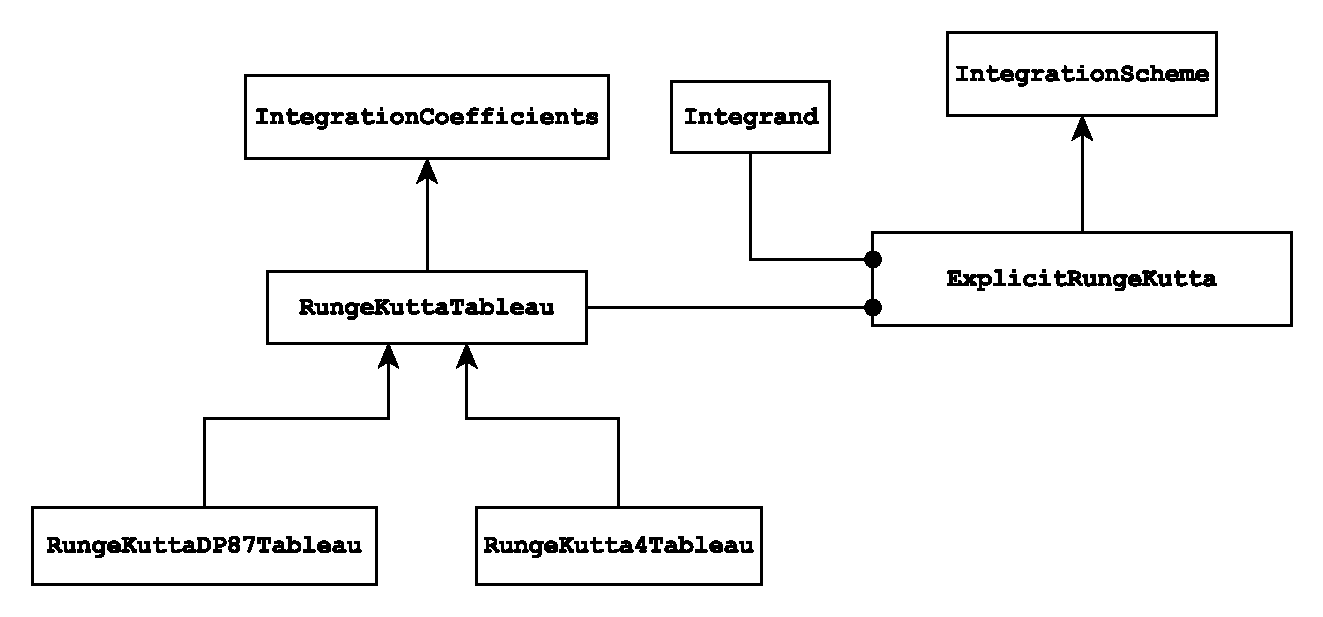
\includegraphics[width=1.0\linewidth]{./integration/IntegrationInheritance.pdf}
    \caption{\label{fig:IntegrationInhseritance} EMTG integration class inheritance diagram.}
\end{figure}

\section{Integrand}
\label{sec:Integrand}
The abstract base \texttt{Integrand} class defines an object that can be numerically integrated by an \texttt{IntegrationScheme} (see \ref{sec:IntegrationScheme}), i.e. it is used to implement a set of differential equations of motion. The \texttt{evaluate} method takes three inputs: 1) a state vector, 2) an input/output state rate-of-change vector, and 3) a bool flag that specifies whether partial derivatives of the equations of motion should be computed. The \texttt{evaluate} method can also be overloaded to accept a control term input. \\

The \texttt{setCurrentIndependentVariable} method sets the current value of the independent variable of integration. For example, the \texttt{ExplicitRungeKutta} class calls this method in \texttt{ExplicitRungeKutta::evaluateIntegrand} immediately prior to calling \texttt{Integrand::evaluate} to ensure that the \texttt{current\_independent\_variable} member variable of \texttt{Integrand} has been updated should it need it. \\

The \texttt{Integrand} class must also populate a \texttt{state\_propagation\_matrix} container, containing the first order partial derivatives of the state differential equations of motion w.r.t. state vector (Jacobian matrix), which can then be retrieved using \texttt{Integrand::getStatePropMat}. 


\section{IntegrationScheme}
\label{sec:IntegrationScheme}

\texttt{IntegrationScheme} is an abstract base class for the numerical integrators in EMTG. The \texttt{IntegrationScheme} class has two constructors. Both require a pointer to an \texttt{Integrand} object that it will integrate, and the one overload also allows the number of integration states \texttt{num\_states} and the state transition matrix dimension \texttt{STM\_size} to be specified on construction.

The primary purpose of this class is to require all of its child classes to define a \texttt{step} method, which integrates the \texttt{Integrand} equations by one step. It also provides the framework for a derived class to define an \texttt{errorControlledStep} for adaptive-step schemes and to compute an associated error via the \texttt{computeError} method.

Prior to calling the \texttt{step} method, the \texttt{setLeftHandIndependentVariablePtr} method must be called to setup the left-hand independent variable of integration (e.g. time, or an orbital anomaly).

The \texttt{step} method takes the following inputs: the left hand state vector and STM matrix (\texttt{state\_left} and \texttt{STM\_left}), output containers for the final integrated state and STM (\texttt{state\_right} and \texttt{STM\_right}), the integration step size (\texttt{step\_size}), the partial derivative of the step size w.r.t. the phase propagation length decision variable (\texttt{dstep\_dProp\_var}) and a boolean variable (\texttt{needSTM}) that determines whether or not the STM variational equations should be integrated (and that is also passed along to the \texttt{Integrand} to inform whether or not it should compute partial derivatives). There is an overload for \texttt{step} that allows for a \texttt{control} vector to be specified.

An \texttt{errorControlledStep} method interface is also provided, which allows for the implementation of a \texttt{step} algorithm that also computes a state/STM error (via \texttt{computeError}) between two integrator solutions of different orders for the purposes of informing an adaptive-step propagator.

\subsection{ExplicitRungeKutta}
\label{sec:ExplicitRungeKutta}

This class implements the explicit Runge-Kutta algorithm for iteratively solving a system of ordinary differential equations. The class is compatible for use with an explicit \texttt{RungeKuttaTableau} of arbitrary order (embedded or otherwise), and computes the first-order variational equations of the system equations of motion. \\

\texttt{ExplicitRungeKutta} defines two \texttt{IntegrationScheme::step} method overrides: one that includes a control vector input, and one without. The \texttt{step} overrides carry out the Runge-Kutta algorithm by calling one of four overloads of \texttt{stageLoop} (with/without control, with/without state transition matrix computations). The \texttt{stageLoop} methods take the left-hand state $\hat{\mathbf{X}}_{n}$ and STM $\hat{\mathbf{\phi}}_{n}$ as inputs and compute the state at the right-hand side of the Runge-Kutta step $\hat{\mathbf{X}}_{n+1}$ as well as the right-hand STM $\hat{\mathbf{\phi}}_{n+1}$ using the \texttt{stateUpdate} and \texttt{stmUpdate} methods respectively (the STM is only computed and updated if the appropriate \texttt{needSTM} flag is passed to the \texttt{step} method). To do this, it computes the first $s-1$ stages using the Runge-Kutta matrix coefficients $a_{ij}$ that it extracts from the class-owned \texttt{RungeKuttaTableau}:

\begin{equation}
\label{eq:X_stage_i}
\mathbf{X}_{i} = \mathbf{X}_n + \sum^{i-1}_{j=1} a_{ij} \mathbf{k}_j ~~~~~ i > j ~~~ i,j = 1,2,3,...,s 
\end{equation}

\begin{equation}
\label{eq:phi_stage_i}
\Phi_{i} = \Phi_n + \sum^{i-1}_{j=1} a_{ij} P_j ~~~~~ i > j ~~~ i,j = 1,2,3,...,s 
\end{equation}

\noindent The specific type of \texttt{RungeKuttaTableau} used is determined at construction time. At each stage, the \texttt{Integrand} $\mathbf{f}$ is evaluated and stored in the \texttt{gradient\_bin} container. Entries in this container are then multiplied by the integration step size in order to compute the stage sub-steps $\mathbf{k}_i$:

\begin{equation}
\mathbf{k}_i = h \cdot \mathbf{f}\left(t_n + c_i h, ~ \mathbf{X}_{i}\right) \label{eq:ith_gradient_step}
\end{equation}

\noindent The matrices $P_i$ are computed as follows, and are stored in the \texttt{STM\_bin} vector of matrices:

\begin{equation}
P_i = \left( \left. \frac{\partial \mathbf{f}}{\partial \mathbf{X}} \right|_{\mathbf{X}_{i}} h + \mathbf{f}\left. \frac{\partial h}{\partial \mathbf{X}} \right|_{\mathbf{X}_{i}} \right) \Phi_{i} \label{eq:ith_STM_gradient_step}
\end{equation}

\noindent In Eq. \ref{eq:ith_STM_gradient_step}, $\frac{\partial \mathbf{f}}{\partial \mathbf{X}}$ is the state propagation matrix that is computed by the \texttt{Integrand} and is retrieved from that object using \texttt{Integrand::getStatePropMat}.

\noindent The Runge-Kutta nodes $c_i$ are used to advance the independent variable of integration, which is represented here as time $t$, but can be any independent variable (e.g. an anomaly if Sundman-transformed equations of motion are being integrated). The final right-hand state, STM, and independent variable are then computed using the Runge-Kutta weights $\hat{b}_i$ 


\begin{align}
\hat{\mathbf{X}}_{n+1} &= \mathbf{X}_{n} + \sum^s_{i=1} \hat{b}_i \mathbf{k}_i, ~~~~~ i = 2,3,...,s \label{eq:ExplicitRKstateStep}\\
\hat{\Phi}_{n+1} &= \Phi_{n} + \sum^s_{i=1} \hat{b}_i P_i, ~~~~~ i = 2,3,...,s \label{eq:ExplicitRKphiStep}\\
t_{n+1} &= t_n + h \label{eq:timestep}
\end{align} 
 
\noindent If the \texttt{ExplicitRungeKutta::errorControlledStep} method is called, then the embedded (lower) order right-hand solution is also computed using the lower order Runge-Kutta weights:

\begin{align}
\mathbf{X}_{n+1} &= \mathbf{X}_{n} + \sum^s_{i=1} b_i \mathbf{k}_i, ~~~~~ i = 2,3,...,s \label{eq:ExplicitRKstateStep_lower}\\
\Phi_{n+1} &= \Phi_{n} + \sum^s_{i=1} b_i P_i, ~~~~~ i = 2,3,...,s \label{eq:ExplicitRKphiStep_lower}
\end{align}

\noindent For an embedded Runge-Kutta routine, the higher order state $\hat{\mathbf{X}}_{n+1}$ and STM $\hat{\Phi}_{n+1}$ are adopted as the solutions on the right-hand side of the Runge-Kutta step (\texttt{state\_right} and \texttt{STM\_right} respectively).


\subsection{IntegrationSchemeFactory}
\label{sec:IntegrationSchemeFactory}


\section{IntegrationCoefficients}
\label{sec:IntegrationCoefficients}



\subsection{RungeKuttaTableau}
\label{sec:RungeKuttaTableau}

The \texttt{RungeKuttaTableau} is a child class of \texttt{IntegrationCoefficients} and defines the Runge-Kutta matrix $A$, weights $\mathbf{b}$, and nodes $\mathbf{c}$ of a particular set of Runge-Kutta formulae.

\subsubsection{RungeKuttaDP87Tableau}
\label{sec:RungeKuttaTableau}

\subsubsection{RungeKutta4Tableau}
\label{sec:RungeKuttaTableau}


